\subsection{choix de la technologie utilisée}
\includegraphics[scale=0.5]{diagrammeDeSequence.png}
\subsection{Représentation de l'information}
\subsubsection{Mot}
Le mot est l'unité atomique de la phrase. Il est représenté par une chaine de caractère sans espace. En français, le radical est la plupart du temps constant dans les mots d'une même famille. Ainsi, il n'est pas nécessaire de changer le radical, mais simplement la terminaison du mot, d'où la nécessité de pouvoir influer sur les quelques dernières lettres en ajoutant ou supprimant celles-ci.
\subsubsection{Phrase}
La phrase est un ensemble de mot, visant à exprimer des concepts. Elle contiendra donc un tableau de mot de longueur indéterminée. A cela s'ajoute la ponctuation finale qui spécifie si la phrase est interrogative ou affirmative. Cette ponctuation finale sera donc aussi stocker en mémoire dans un caractère dédié. Le sens d'une phrase étant définit par certains mots tels que pronoms et verbes, il est nécessaire de pouvoir parcourir la liste de mot ou de pouvoir savoir si tel mot est présent dans la phrase.
Enfin, afin de créer une réponse sensé, il est nécessaire de pouvoir créer une phrase en s'appuyant sur les mots de la phrase précédente.
\subsubsection{Robot}
En français, la position de chaque mot est importante car elle a une influence sur la phrase. La grammaire française est une grammaire complexe. Cependant, contrairement à l'allemand, la position des mots n'est pas absolument figé, et grâce au virgules notamment, il est possible de séparer le sujet de son verbe. Le succès des robots dans ce domaine reste encore très limité, et faute de temps et de moyens, nous nous limiterons au traitement de phrase simple, avec un sujet précédant directement son verbe.

\begin{figure}
    \center
	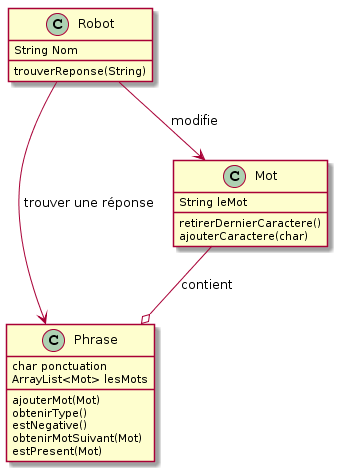
\includegraphics[scale=0.5]{diagrammeDeClasse.png}
	\caption{Diagramme de classe}
\end{figure}
